\section{Introduction}
\label{sec:intro}

With the end of Moore’s law and Dennard scaling, developers are forced to distribute their applications to process an ever growing amount of data. As a result, the past decade has seen a proliferation of new distributed frameworks~\cite{kubernetes, ray-osdi, mesos} to handle a variety of workloads from big data (e.g., batch jobs, interactive query processing) to AI applications (e.g., model training and serving).


% https://docs.google.com/drawings/d/1jXbZJhnhrtNHtrjuyGhHoiT4LbjzwVerwn02Tnw-Kv0/edit
\begin{figure*}[ht]
\centering
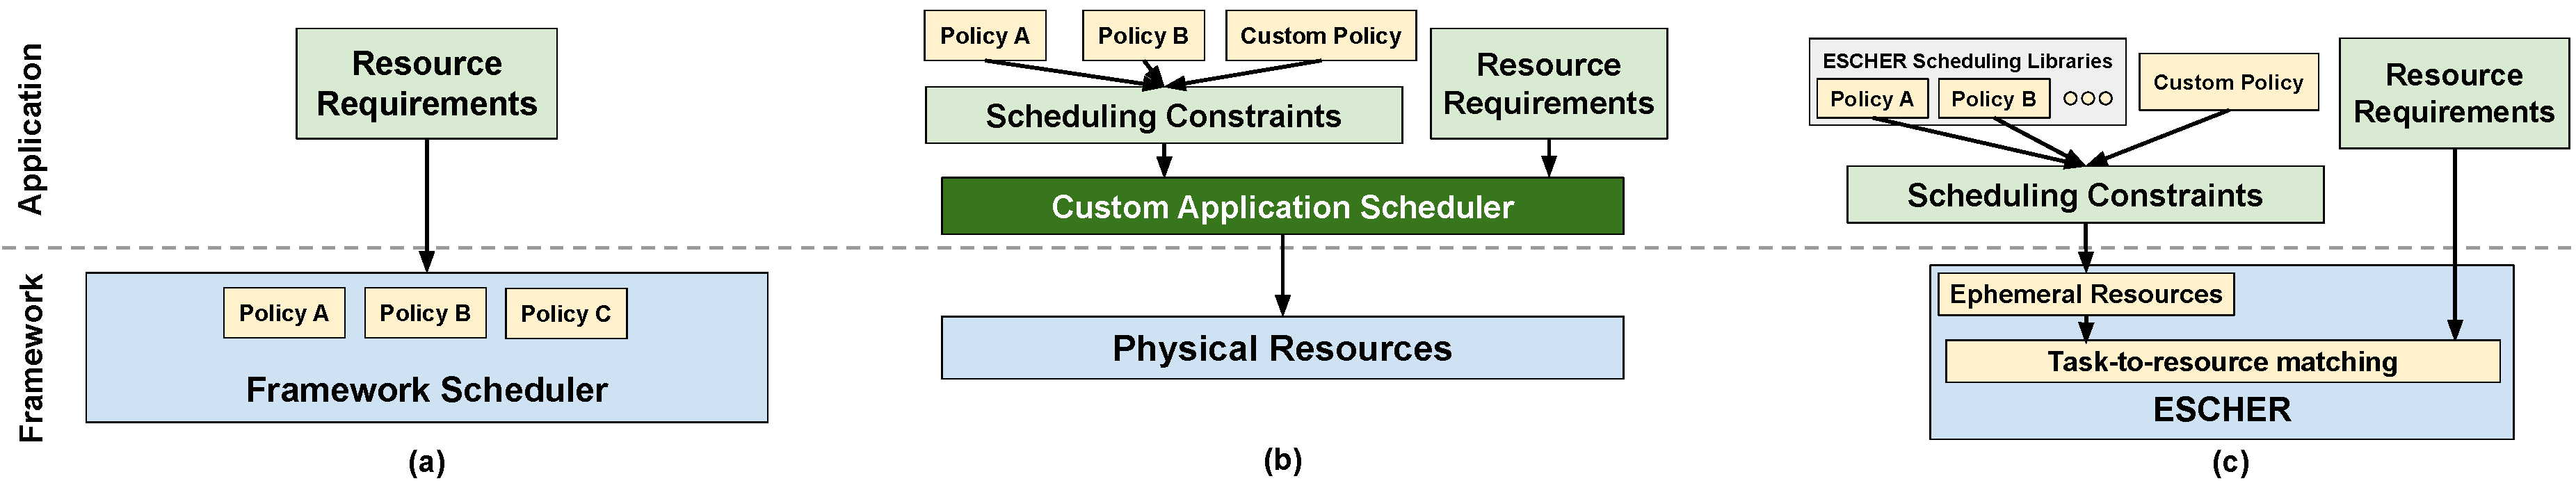
\includegraphics[width=0.92\linewidth]{escher/figures/escher-compare-arch.pdf}
\caption{\small
\textbf{(a)} A monolithic scheduler implements both scheduling and resource constraint matching~\cite{ghodsi2011dominant,isardquincy,mpi,kubernetes}. Some schedulers allow applications to express and compose certain policies~\cite{condor,tetrisched,kubernetes}, but custom application policies may require modifying the scheduler itself.
% Though this API abstracts away scheduling logic from the application, it is not expressive enough to allow applications to express compositions of scheduling policies.
\textbf{(b)} To maximize flexibility, some frameworks expose physical resources \cite{mesos, omega}, but require applications to write custom schedulers that manage both policy and resource coordination~\cite{gandiva,DevinMasters,mapreduce}.
%This burdens the application developer with explicitly handling resource allocation.
\textbf{(c)} \name{}. With ephemeral resources, applications can express custom policies through ephemeral resources, while the cluster scheduler provides just one service - satisfying per-task resource constraints.
}
\label{fig:scheduler-architectures-new}
\vspace{-2mm}
\end{figure*}

% Introduce evolving policy requirements
As the number of data and AI applications grows, so do their scheduling requirements. 
%Different applications demand different scheduling policies from these frameworks. 
Some examples of scheduling policies are \emph{affinity} (i.e., co-locate computation with data to avoid costly data transfers), \emph{anti-affinity}  (i.e., schedule tasks on different machines to avoid interference), 
%\emph{load balancing} (e.g., distribute requests round-robin across multiple servers), 
and \emph{gang scheduling} (i.e., schedule a group of interdependent tasks simultaneously). For example, a hyperparameter search application~\cite{hypersched,gandiva} consists of multiple distributed training jobs, each consisting of multiple parallel tasks. This requires anti-affinity between jobs for high throughput, affinity within a job to avoid unnecessary data transfers, and gang scheduling to ensure multi-node jobs are not starved. 
%Worse yet, some of these application policy demands emerge after the scheduling framework has been released.

% Current scheduling landscape
This diversity of policy requirements makes designing schedulers for distributed frameworks challenging. There is an inherent trade-off between \emph{simplicity} and \emph{flexibility} in exposing different policies to applications. Different cluster managers occupy different points in this trade-off space. 

At one end of the spectrum (Figure \ref{fig:scheduler-architectures-new}a), monolithic cluster managers like YARN~\cite{yarn} and Kubernetes~\cite{kubernetes} provide several out-of-the-box policies for the application to chose from. This simplifies the application's task, but it compromises the flexibility, as adding a new policy requires changes to the scheduler and the cluster manager itself. Implementing a new policy requires the developer to understand and modify the source code of the cluster manager, not always an easy task given their inherent complexity. And, once the new policy is implemented, the developer is on the horns of a dilemma: either fork the project and pay the cost of maintaining it up-to-date as the project evolves, or wait many months for the change to be merged in the main branch. Worse yet, if the cluster manager is closed source, the application developer has no choice but to wait and hope that the company behind the cluster manager will implement the desired policy.

At the other end of the spectrum (Figure \ref{fig:scheduler-architectures-new}b), are schedulers like Omega~\cite{omega} and Mesos~\cite{mesos} that enable an application to directly allocate resources and implement its own scheduling logic. This makes these cluster managers very flexible, but dramatically increases the complexity of the application. Implementing a scheduling policy in a distributed system can be a daunting task, as it requires not only allocating resources, but tracking the resource availability in the presence of various failures and new nodes joining the system.

%Moreover, keeping the fork of the source code up-to date with the upstream master branch can be tedious and requires constant maintenance.
% Explain why this landscape is not sufficient
%The cluster managers in the first category simplify the applications by implementing the entire scheduling logic, but compromise the flexibility, as adding a new policy requires changes to the scheduler and to the cluster manager itself. 

%Implementing a new policy requires the application developer to understand and modify the source code of the cluster manager. This requires in-depth knowledge of the cluster manager which the developer might not be familiar with. Moreover, keeping the fork of the source code up-to date with the upstream master branch can be tedious and requires constant maintenance. Cluster managers in the second category are highly evolvable, as the applications can implement any scheduling policy they want. This comes at the cost of complexity, as implementing a scheduler in a distributed system requires not just allocating resources to tasks, but also tracking resource availability in a distributed, fault-prone environment.


% Introduce virtual resources
In this work, we present another point in the design space that allows application developers to easily implement a range of new scheduling policies. This design point is enabled by a mechanism recently introduced by cluster managers like Kubernetes and Ray which provides an interface for applications to dynamically create, modify, and destroy logical resources. We call these resources \emph{ephemeral resources}.  Like regular resources, ephemeral resources are pairs of labels and count values which can be allocated to tasks. The scheduler treats ephemeral resources in the same way as physical resources, subjecting them to admission control to ensure they are not oversubscribed. This frees the applications from performing admission control and tracking availability.

%Interestingly, in addition to these mechanisms, some cluster schedulers provide an interface for users to dynamically create and modify \emph{virtual} resources on physical nodes in the cluster. Like regular resources, \emph{virtual} resources are pairs of labels and count values which can be allocated to tasks. For instance, in Kubernetes and Ray, users can create resources on nodes to identify specialized accelerators (e.g. {Nvidia V100 GPU: 4}). These virtual resources can then be requested by tasks, and the cluster scheduler ensures that tasks are placed on nodes where resources are available. The cluster scheduler treats virtual resources the same as physical resources, subjecting them to admission control to ensure they are not oversubscribed. 

% Give example of scheduling with ephemeral resources
We find that a surprisingly large number of scheduling policies can be expressed by dynamically creating, updating and destroying ephemeral resources. Consider a simple scheduling constraint to colocate two tasks T1 and T2. To express this constraint, an application would submit T1, which creates an ephemeral resource R1 during execution, and then submit T2 with R1 as a resource requirement. The scheduler is then forced to place T2 on the same node as T1, since no other node has resource R1. While this is a very simple example, it illustrates the underutilized power of ephemeral resources for satisfying application-level scheduling constraints. In contrast, a monolithic cluster manager would have to expose a primitive designed specifically for task-task affinity, and a two-level scheduler application would have to implement the entire policy themselves, choosing where \emph{both} T1 and T2 execute.

% Raise the thesis of this paper
%This raises a natural question - by dynamically creating ephemeral resources and requesting them in task resource requirements, can applications express and satisfy their scheduling constraints? In this paper evaluate this question through the lens of generality (can ephemeral resources satisfy a wide range of scheduling constraints?), performance (is scheduling with ephemeral resources as performant as modifying the core scheduler?) and simplicity (how easy is it for applications to use ephemeral resources?).

%\ion{This is the key paragraph that must state super clearly why emphemeral resources are useful and what are the questions we want to answer in this paper.} 
The key promise of ephemeral resources is that they enable an application to implement new scheduling policies \emph{not} supported by the underlying cluster manager. This increases the velocity of deploying and iterating on new application functionality. % and thus reduces the time to value for new products and features.
However, there are two natural questions that follow. First, how general are the scheduling policies enabled by ephemeral resources? Second, what are the costs in terms of implementation complexity and overhead compared to natively implementing the same policy in the cluster manager?
After all, if these overheads dominate, then an application developer is better off building their own scheduler.

To answer these questions, we propose a scheduling architecture for distributed applications called ESCHER \footnote{\name{} stands for Expressive SCHeduling with Ephemeral Resources.}.
In ESCHER, the application uses ephemeral resources to implement its scheduling policy instead of relying on the cluster manager's baked-in policies.
The key insight of ESCHER is that a broad class of heterogeneous scheduling constraints can be cast as \emph{ephemeral resource requirements}. The underlying scheduler simply enforces these requirements. ESCHER enables applications to implement a large number of scheduling policies by (1) dynamically creating new ephemeral resources, and (2) specifying task resource requirements on these ephemeral resources. We find that by using these two simple primitives, we are able to satisfy a large set of scheduling constraints, without requiring any changes to the core scheduler or significantly affecting application performance. For instance, gang-scheduling in ESCHER can be written in 10x fewer lines of code with less than 2x overhead in scheduling latency compared to implementing the policy natively in the core scheduler (\cref{sec:eval:gangscheduling}).

%\romilc{The reason \name{} simplifies implementing new policies at the application level is because the core scheduler fulfills a singular responsibility - satisfying a task's resource demands (ephemeral and physical).
%This responsibility implies that only resource tracking and coordination (resource acquisition and release) be implemented by the core scheduler.
%The application satisfies its scheduling constraints by specifying per-task ephemeral resource requirements and manipulating these ephemeral resources over the lifespan of the application.}
%Effectively, \name{} enables a broad class of \textit{heterogeneous scheduling constraints to be cast as ephemeral resource requirements}. 

% Tradeoffs with ephemeral resources.
However, the flexibility of ephemeral resources does not come for free. First, it increases the application complexity compared to monolithic schedulers in which applications just need to select one of the available policies. Implementing certain policies, such as gang scheduling, requires the application to implement additional mechanisms using ephemeral resources such as ghost tasks, i.e., tasks whose sole purpose is to signal when all required resources have been allocated. Second, because ephemeral resources are created dynamically, an application must handle infeasible requests explicitly. For example, if a task's resource request cannot be satisfied, the task will hang and it must be explicitly terminated.% the application must explicitly terminate it. 
%Second, ephemeral resources need to be \emph{handled with care}. In cases when an application makes a request of ephemeral resources that is not feasible, the application might have to roll back and free the ephemeral resources it has allocated.  This is akin to the way memory management (malloc, free) is handled in many low-level programming languages. 
% Finally, debugging is challenging as it requires logging and replaying the ephemeral resource creations and deletions.
%Finally, since ephemeral resources are declarative in nature, debugging them requires replay of resource creation/deletion logs, which can be challenging.

% Second, because the ESCHER architecture provides no visibility into the global cluster state, tasks in multi-tenant environments have slightly reduced performance due to the back-off based collision avoidance in ESCHER.

% Tradeoff mitigation
%which reduce implementation burden of applications for common policies.
To alleviate the challenge of application complexity and provide protection against invalid resource specifications, ESCHER supports  simple libraries to support common policies. We call these libraries \name{} Scheduling Libraries (ESLs). ESLs aim to provide the best of both worlds: the simplicity of monolithic schedulers, and the flexibility of adding new scheduling policies at the application level by either extending an existing ESL or creating a new one. ESLs decouple application logic and policy by abstracting ephemeral resource management for common high-level scheduling policies, thus dramatically reducing development cost via code reuse and enabling composition of simple policies into more complex ones. % ESLs compose with other ESLs as well as custom policies. %Thus, ESLs offer the benefits of modularity, such as policy composition and reuse, while still allowing applications to implement custom policies. 
%As the name suggests, ESLs are akin to libraries in today's programming languages which implement the most common functionality and expose it to developers through simple APIs, thus dramatically reducing development cost via code reuse and enabling composition of simple policies into more complex ones.

%To evaluate \name{}, w
To evaluate \name{}'s performance, we implement it on both Kubernetes~\cite{kubernetes} and Ray~\cite{ray-osdi} by leveraging their existing implementations 
%\swang{was it existing for Ray? I thought that we implemented it for this paper}
% of ephemeral resources.
for label-based scheduling, which were originally intended to represent custom physical resources rather than logical scheduling constraints.
We run \name{} on a range of applications and policies, including  WordCount MapReduce with max-min fair sharing on Kubernetes as well as
AlphaZero~\cite{silver2016alphago} and distributed model training on Ray~\cite{ray-osdi}. We show that \name{} does not impact the end-to-end performance of most applications when compared to a system that implements the same policies in the core scheduler. Meanwhile, the application can use \name{} to express additional policies not supported by the underlying core scheduler, e.g., composing gang scheduling with affinity~(\Cref{sec:eval:tune}). %increase the completion times of some applications, e.g., applications consisting of sub-millisecond level tasks. 
%\ion{I find the point that we can use ESCHER to implement the policy in the core scheduler confusing. I'd just say that in some cases there is overhead and give one or two examples of such cases.}
%\romilc{While the performance of \name{} is largely comparable to policies hard-coded in a monolithic scheduler, the application-level mechanisms used to implement policies can add to the scheduling latency for some workloads. However, if performance is a priority, ESCHER can also be used to implement policies at the system level by modifying the core scheduler. In \Cref{sec:eval}, we evaluate the tradeoffs involved in moving policies to the system level.}
%In the process, we show that \name{}~is able to match the performance of comparable policies hard-coded in a monolithic scheduler.

Thus, \name{} shows that one can take advantage of the ephemeral resource abstraction, whose implementation is already partially provided by some cluster managers, to express a surprisingly diverse set of scheduling policies at the application level without having to touch the core scheduler. This allows users to quickly implement new policies, as needed, to improve support for their applications.

% To reiterate, the main point of this paper is not to claim that implementing a scheduling policy using ephemeral resources is better than implementing it in the cluster's core scheduler, or that it is the best mechanism to implement an extensible scheduling architecture. Rather, our goal is to show that one can take advantage of the ephemeral resource abstraction already provided by existing cluster managers to implement a surprisingly diverse set of scheduling policies at the application level, without having to touch the core scheduler. This allows users to quickly implement new policies, as needed, to improve support for their applications.

%Effectively, \name{} trades a small loss in performance in favor of significant increase in the flexibility of the scheduler to support new policies.
In summary, we make the following contributions: 

\begin{compactitem}
    \item \name{}, a scheduling architecture that uses ephemeral resources to express scheduling policies without modification to the core scheduler.
    % \item An evolvable scheduler design that uses a simple resource-matching scheduler, allowing applications to express policies with ephemeral resources.
    % \item We show that ephemeral resources can support existing policies with little performance degradation completely in the application space.
    \item Design and implementation of a wide class of scheduling policies (\S\ref{policies}) using the ephemeral resources API.
    % \item Support for new policies through \emph{dynamic} creation and destruction of ephemeral resources.
    % \item We show that it is possible to implement a general scheduler and to express policies in the application space, including dynamic and composed policies, with one simple abstraction, ephemeral resources, and one simple mechanism, task-to-resource matching.
    \item ESLs: application-level scheduling libraries that enable applications to easily compose and re-use policies.
    % \item We show that policies implemented by the applications with ESCHER can match the performance of equivalent policies implemented natively by the framework. % The resource management is still handled by the framework 
\end{compactitem}





% 1. Put the sentence at the start of the - despite these tradeoff, ephemeral resources are the only method that provides the user ability to implement besides modifying the core scheduler for dominant monolithic schedulers. .

% 2. "We find that a surpsingly" comes too late. Maybe add that before you introduce the mechanism. Another point in the design space. 

% Ephemeral resources. 
% Virtual -> Logical
% Epheemeral resources are dynamic short-term resources. Can be programatically created and destroyed.

% Debugging is challenging because you don't know when resources are created and deleted. 

% ESLs - If I have a ESL, why not in core scheduler?
